% \section{Conclusions and Open Challenges}

% massive expenditure required for wide deployment of new services 


% In this thesis, we tackled a number of issues 
% In this thesis we argued that the conventional approaches towards optical access network infrastructure ownership will not be capable of supporting the emerging heterogeneous services. We have shown that the best practise for sustainable deployment of the next generation of network services inevitably involve heterogeneous network where the network infrastructure is shared among many service providers. Therefore unlikely that the handfull of telecommunication conglomerates to be able to raise the capital requied for this massive upgrade in their infrastructure and therefore new network ownership models will emerge. 
% Such network ownership models rely on the oerators' ability to coexist and cooperate on the same physical infrastrusture and it is critical for them to not to interfere with each other's operation. We have shown that current hardware focused network equipment and standards do not allow for the flexibility required for such scenarios. These limitations include the network functions such as capacity scheduling which greatly influence the network's \acp{KPI} which in case of the new multi-service networks will not nessecarily be alligned among all the operators.

% Multi-dimensional growth of demand for networks penetration both in number of people connected and ratio of device each, widespread use of multimedia content and diversity of day to day tasks that rely on networks. Therefore the new generation of mobile networks 5G has put the efficient transport network in top of their agenda as this constructs a significant part of their costs.
% The sharing is inevitable 

The core objective of this thesis was to explore the potential of network sharing in the context of optical access networks, first, to assess the presence of motivations to adopt fine-grained active sharing. Second, to identify the technical and economic barriers that could prevent the stakeholders from embracing network sharing despite the intuitive motivations. And finally, to address these barriers using state-of-the-art technical and economic solutions. The high-level outline of this thesis is depicted in \autoref{fig:outline}.

\tochange{Update \autoref{fig:outline} at the end}
\begin{figure}[tbhp]
\centering
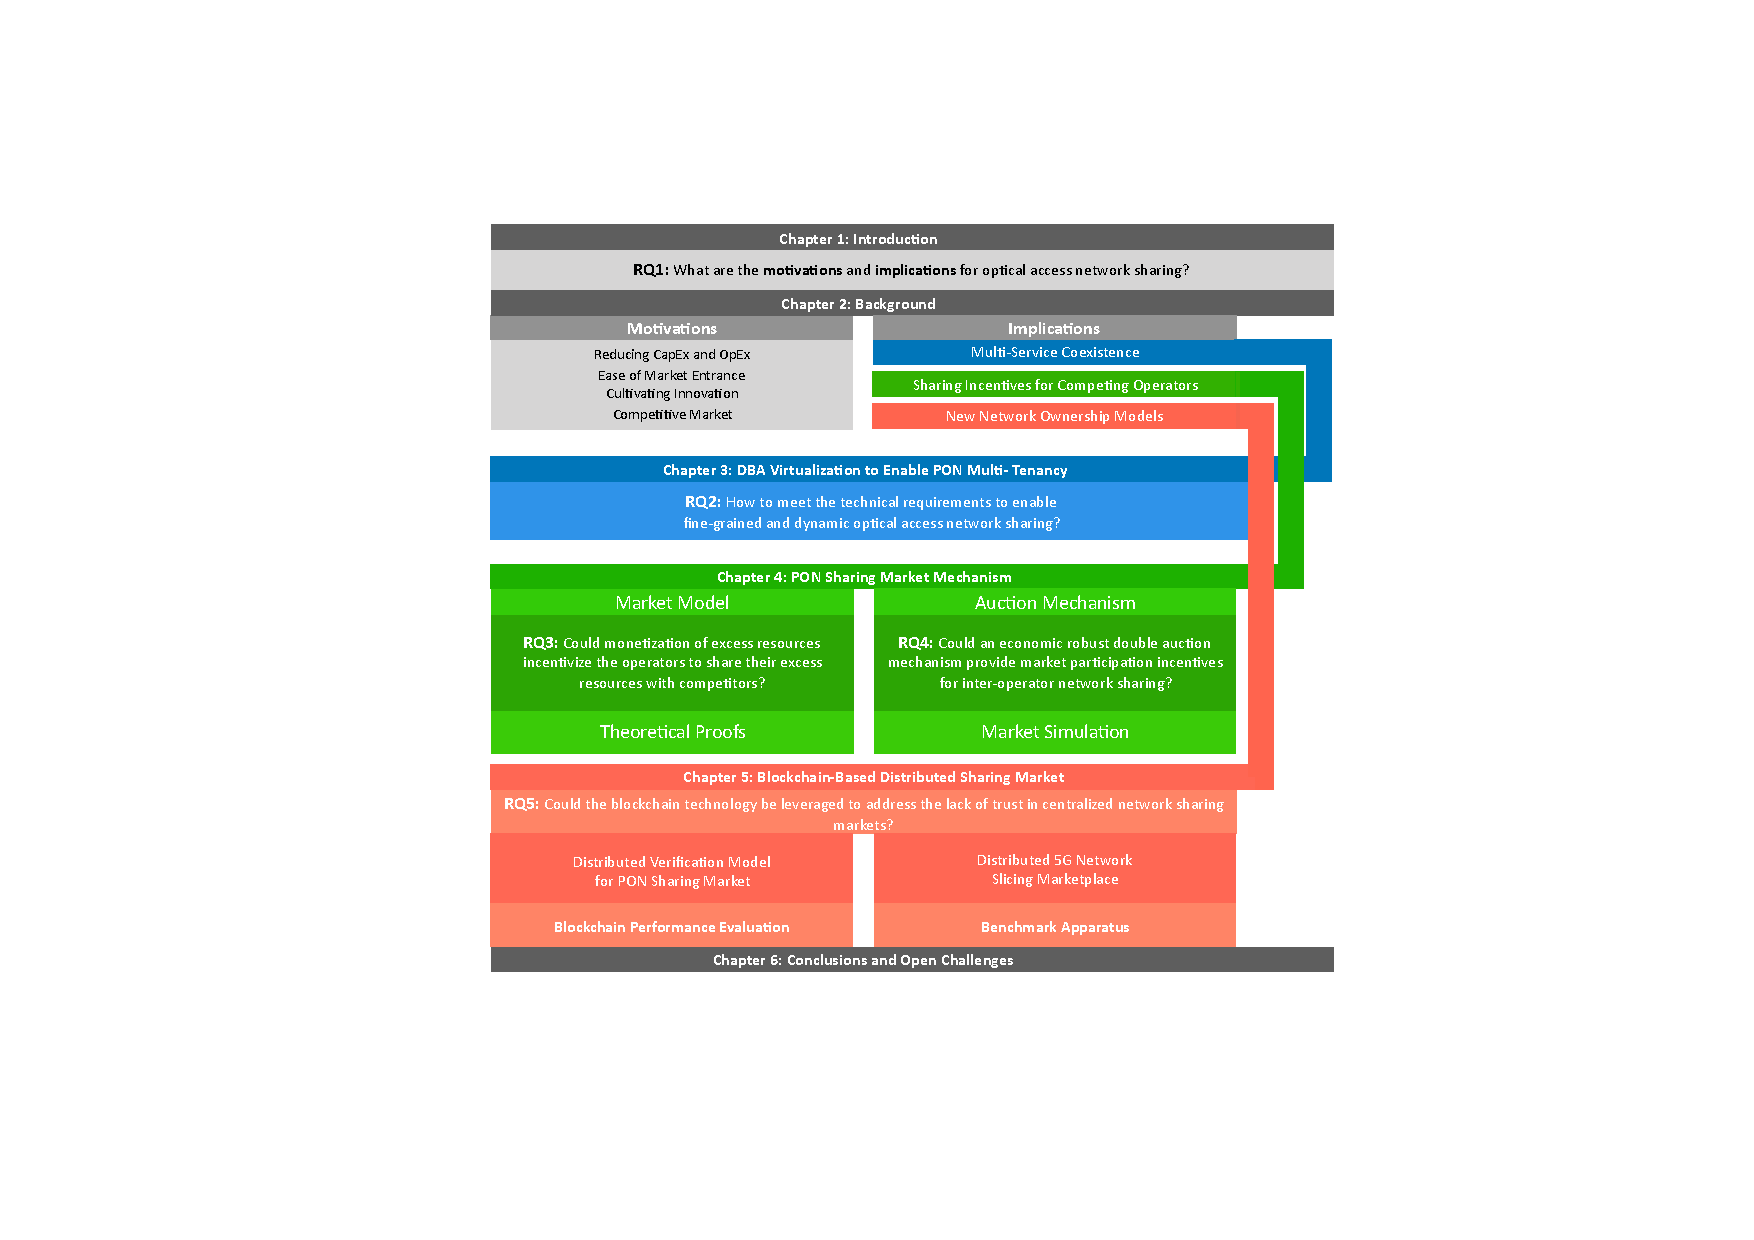
\includegraphics[width=\linewidth]{Figures/outline.pdf}
\caption{The Dissertation Outline}
\label{fig:outline}
\end{figure}
\section{Summary}
In \autoref{cpt:background}, we provided an overview of the background as well a review of the state-of-the-art literature on the underlying concepts related to this dissertation. By doing so, we identified the motivations for optical access network sharing which included reducing total network expenditure and market barriers for new and smaller service providers, cultivating innovation and encouraging competition in the communications market. Therefore we answered the first part of the Research Question 1: \textit{\RQa}. Regarding the second part of RQ1, three major implications arose, one technical and two economic. First, the technical implication of multi-service coexistence of network operators over the same physical infrastructure. Second, the lack of sharing incentives for competing operators and third, the emerging network ownership models that are expected to disturb the balance of the conventional approaches in the communication networks' market. These implications then became the main theme of this thesis, producing RQ2-5.

% In \autoref{cpt:methodology} we introduced the methodology used to evaluate the proposed answers to the research questions. We showed how we prove the economic robustness of the market mechanism of optical access network sharing. We described the market simulator used to collect data on the utility distribution of the market players, overall social welfare of the market and the network utilization. In \autoref{cpt:method:sec:bc} we described the evaluation process of the distributed market application including the \acp{KPI} such as transaction throughput, latency and computing intensity. We further elaborated on the benchmark apparatus used to design the experiments and generate the results. And finally, we explained how the pragmatic experimental Blockchain deployment contributes to the accountability of our results compared to the state-of-the-art work.


In \autoref{cpt:chapter_1} we provided an answer to Research Question 2: \textit{\RQb}. We leveraged network virtualization technology to tackle the inflexible nature of the \ac{DBA} algorithm that were not capable of supporting heterogeneous services due to the orthogonal performance requirements. We demonstrated how this inflexibility was a technical barrier to multi-service coexistence in \acp{PON}. We proposed the concept of \ac{vDBA} that would allow the \acp{VNO} to operate their desired instance of upstream capacity scheduling thus meeting their service-specific \ac{QoS} requirements. We finally described how the lack of economic sharing incentive for sharing the excess capacity among these operators motivated the RQ3.


In \autoref{cpt:chapter_2} we addressed the Research Question 3 that was raised in the previous chapter. RQ3: \textit{\RQc} We modeled the multi-tenant \ac{PON} as a two-sided market where the \acp{VNO} with excess capacity can trade their resources with others in return for monetary compensation. We formally defined how the \acp{VNO} would valuate their excess capacity in such a market and how different strategies could affect their utilities in the market. Next, we acknowledged that in the absence of a manipulation-proof market mechanism the \acp{VNO} would use manipulative strategies to maximize their own profit without considering others' utilities. We argued that such a behavior would lead to distrust among the \acp{VNO} and eventually lack of trading activity. In response to Research Question 4: \textit{\RQd}, we propose a double auction mechanism that provides a matching between the seller and buyer \acp{VNO}. We used mathematical proofs and market simulation methodologies introduced in \autoref{sec:Auc:methodology} to assure the economic-robustness of the proposed auction mechanism. Furthermore, we compared the proposed mechanism with an state-of-the-art mechanism and the results showed up to $\approx 40\%$ improvement in terms of allocative efficiency (social welfare). 
% \vspace{-1mm}

In \autoref{cpt:chapter_3}, we presented an alternative approach to the centralized conduct of the resource sharing market where no central entity is trusted by all the parties to manage the market. This new approach provides the answer to the Research Question 5: \textit{\RQe}, We used the blockchain technology to develop a distributed market-place that relies on a collaborative consensus rather than centralized control. The auction mechanism is implemented as a smart contract which requires all (or a subset) of the market players to endorse and verify the transactions occurring as the result of the auction. This smart contract once agreed upon is immutable the same way that all the transaction information recorded on the distributed ledger are immutable. Furthermore we acknowledged that replacing the centralized market management with a distributed approach will impose certain overheads to the system. To further explore, we used the blockchain evaluation methodology introduced in \autoref{sec:BC:methodology} to study the feasibility of using the distributed market in two communication network scenarios. First, we proposed to enhance the multi-tenant \ac{PON} market introduced in \autoref{cpt:chapter_2} with a verification layer that is deployed on the blockchain and uses the distributed market mechanism to produce an auditable record of the \ac{PON} auction transaction. Second, we addressed the 5G slice brokering problem. We replaced the centralized brokering of slices among different network operators with the blockchain-based distributed market mechanism. We designed pragmatic experiments to evaluate the performance of the distributed market mechanism under varying transaction send rates. The results of this study indicated that our proposed market mechanism can process up to 40 and 100 transactions per second with respectively no and negligible loss in transaction throughput. Meanwhile the average transaction latency under varying send rates remained under 1 second. These finding suggest that considering the slice brokering trade frequency that is expected to be conducted on a minute scale, our proposed distributed market could support the ecosystem without imposing significant overhead.




% \vfill
\section{Open Issues and  Future Work}
In this thesis we made several contributions concerning the technical and economic challenges of optical access network sharing. In the following we provide a number of open challenges including extensions to the contributions of this thesis and potential research ideas inspired by the topics addressed in it for some of which future work is already underway by the author.



% The proposed distributed market mechai These soulution could be applied to other
%  the results in this thesis also provide a strong foundation for future work
 
% The research presented in this thesis seems to have raised more questions that it has answered. There are several lines of research arising from this work which should be pursued.


% Future work concerns deeper analysis of particular mechanisms,
% new proposals to try different methods, or simply curiosity.



% \subsection{IRC Proposal}
\subsection{Comprehensive Blockchain Performance Evaluation Methodology}% for Communications solutions}
Provisioning the required resources for a blockchain-based distributed application depend tightly on one's ability to precisely evaluate the performance of a blockchain network. As mentioned in \autoref{sec:BC:methodology} blockchain's performance can be affected by a number of parameters. These Parameters include block size, the choice of key-values world state database (GoLevelDB vs. CouchDB), the geographical distribution of the blockchain peers, the endorsement policy, and the consensus protocol. However, we regarded the comprehensive investigation of this parameters outside the scope of this thesis. 
Therefore a future work can identify and elaborate on the performance metrics associated with blockchain applications and determine how these metrics affect the resource provisioning in terms of computing, network or memory costs. 
The outcome of this work could be a comprehensive methodology for feasibility and cost analysis of a blockchain application with a focus on application in the telecommunications area. This methodology would be of interest for a broad range of researchers and industries who are focusing on designing blockchain-based solutions.


% decentralising a current centralised telecommunications process using blockchain technology. Blockchain and smart contract technologies offer trust and fault tolerance to record-keeping and function enforcement processes by introducing an overhead to the functionality of the system. For instance, the fault/manipulation tolerant record-keeping feature offered by blockchain entails that every record that is to be written on the database has to go through a rigorous process of verification until all the participants reach a consensus on the final value of the record. Therefore, compared to a centralised database, it takes considerably more time/resources to write a record on the blockchain. Furthermore, an overhead computing cost is introduced to the process. Therefore it is essential to precisely measure these overheads and take them into account while designing a blockchain solution. This becomes more critical for telecommunications use cases since latency is of utmost importance in the fifth-generation (5G) mobile networks. 
% Therefore a future work could target to formulate design guidelines for telecoms blockchain solutions based on performance metrics and resource costs. The blockchain framework of choice for this research is the open-source Hyperledger Fabric platform which is specially designed for enterprise ecosystems. Hyperledger Fabric offers numerous advantages compared to the other alternatives (e.g., modular design, high throughput, and multi-language smart contract support). A Linux Foundation working group is dedicated to studying Hyperledger's performance and scalability. The results of their study are published as a white paper [1] introducing the blockchain system-specific performance metrics. These include quantitative metrics that measure the performance of the blockchain and in particular, the execution of the smart contracts. The smart contract is the logic behind any blockchain application, where the participants can invoke certain transactions. If the proposed transaction successfully passes the consensus and verification phase, it will lead to writing a record on the blockchain. The primary performance metrics introduced in the literature include 1) Transaction Throughput (how many transactions can be processed per second), 2) Transaction Latency (the time it takes to process a transaction), and 3) Computing Intensity (the computing resources required such as CPU, memory, and network). In [2], the authors have studied the impact of different blockchain network design decisions on the performance of the application (e.g., number of channels, state database technology, and block size). Depending on the type of application, and the ecosystem, the requirements for these metrics could vary. For instance, in an inter-operator resource sharing market where the frequency of transactions is very high, the transaction latency becomes the most critical factor. On the other, in applications such as the Internet of Things (IoT), the computing intensity of the blockchain operation would be a bottleneck in designing solutions (due to the resource limitation of IoT nodes). This is in-line with my research as I aim to identify similar metrics. However, I will focus on identifying further factors that step beyond the generic stress test metrics and discover telecoms-specific performance determinants. 
% A growing body of scientific literature is dedicated to the study of use cases where blockchain and smart contract technologies could be leveraged to address various issues. These issues include trustless enterprise ecosystems, security/privacy concerns, supply chain management and industrial automation in a wide range of disciplines including finance, telecommunications, health care, etc. While many of these research use cases are very promising, often, the performance and cost implication of redundancy imposed on the system by using blockchain is overlooked. The study of the performance and cost is essential to the development and feasibility analysis of a blockchain application as these could easily become a bottleneck and cancel out the advantages of the blockchain and lead to the impracticality of the solutions. 

% - In this research, I intend to propose a performance and cost evaluation methodology to allow precise investigation of the consequential redundancy imposed on the system by the blockchain. The performance and cost evaluation method would be of interest for a broad range of researchers and industries who are focusing on designing blockchain-based solutions. The potential outcome of this research will influence design decisions when developing blockchain applications. 

% - The technical implementation details covered in my scientific publications as well as the tutorial content I regularly publish online on popular websites such as LinkedIn and Medium can inspire further research in the area and also reach a broader audience beyond academia. These articles incorporate technical reports on blockchain application development, automated container orchestration, and cloud networking. 

% - The distributed market mechanism designed throughout this research will focus on optical network infrastructure market. However, a significantly broader range of use cases within and outside the communications sector can adopt before-mentioned market mechanisms to enable trade in trustless environments. For instance, wireless network slicing or high-frequency stock trading markets where similarly, multiple traders in both sides of the market want to trade commodities without relying on a central trusted authority.

% \subsection{combinatorial auction}

\subsection{Automatic \ac{SLA} Enforcement using Smart Contracts}% of  agreements using smart contract technology for multi-operator communications infrastructure}
\acfp{SLA} between network operators and infrastructure providers could play an integral role in network sharing. The \ac{SLA} has to provide a detailed description of the expected reliability, availability and other performance metrics of the service and the actions to be taken in case of one of the parties breaching the agreement (i.e., the supplier not meeting the terms of the \ac{SLA}). However, the enforcement of these \acp{SLA} remains an open challenge as manual enforcement and conflict resolution could become a bottleneck in the highly dynamic network sharing scenarios. Future work is already planned by the authors to first identify the \ac{SLA} processes that could benefit from automation and second to investigate the possible implementation of this processes as smart contracts to facilitate automation. These smart contracts would trigger certain transactions based on the negotiated terms of agreement and keep a tamper-proof record of them on the blockchain ledger.



% investigations are necessary



% no automated process has been proposed to address the problem. In the next section, we will discuss how smart contract technology can provide an automatic approach towards enforcement of \acp{SLA}.


% This paper will also define additional transactions to be triggered in case of an agreement breach. These pre-negotiated agreements set out certain transactions (e.g., a penalty of transfer of fees) when a particular term in the agreement is not met.

% to identify the certain processes that become a bottleneck due to manual enforcement and conflict resolution. Then, I will exploit the smart contract technology to enable automatic enforcement of the terms of agreements. For instance, these agreements might include Quality of Service or service availability guarantees. In such circumstances, a penalty often is pre-negotiated and manually enforced in case of breach of the agreement. The smart contract technology can, therefore, be used to assure automatic enforcement of the terms (e.g., financial penalty etc.) As mentioned in the proposed plans section, The results of this research will be submitted to the Journal of Lightwave Technology (JLT).


% The second publication aims to provide a distributed mechanism to operate automated transactions in inter-operator markets in the telecoms sector. A large volume of literature has addressed designing centralised market mechanisms (mainly auctions) using game-theoretical approaches [3]. However, due to the lack of a trusted central authority to conduct the auction, centralised mechanisms and models are not eligible for solving the trust issue among the network operators. Authors in [4] have proposed using blockchain for peer to peer energy trade and concluded that their distributed auction promotes better the local trading of energy than a centralised version. However, they rely on simulation as their methodology to evaluate the performance of their system. The evaluation in my setup will be performed in a practical industrial blockchain framework, the Hyperledger Fabric, where the network architecture resembles a production-grade deployment. Furthermore, I will deploy a Byzantine fault-tolerant consensus protocol called RAFT to assure uninterrupted functionality of the blockchain operation in case of a peer failure. 
% \subsubsection{Quality Assurance and Enforcement}

% A slice of the network comes with certain qualitative guarantees, often in the form of a pre-negotiated \ac{SLA}.  The authors in \cite{SLA-Slicing} have introduced a number of metrics regarding the slice-based network \acp{SLA} including throughput, penalty, cost, revenue, profit, and QoS related metrics.



\subsection{Distributed Data-Sharing Governance for Optical Networks}
% Project Title: Distributed Data-Sharing Governancev for Optical Networks
% Objectives: 
The autonomous operation of data-driven optical network management relies on the development of trusted interaction among all participants. For example, given the set of all available monitoring information, different parties should only have access to specific subset of the data, depending on their role (e.g., infrastructure provider, virtual operator, slice provider, end user, etc). Future work could investigate the issues associated with the governance of multilateral data-sharing in optical networks. A distributed market mechanism similar to the one proposed in \autoref{cpt:chapter_3} could be used for data monetization using a credit-based system to incentivize sharing of the data. Furthermore, the access Control mechanisms available in blockchain platforms could be leveraged for identity management and authorization in data governance.
\vfill


% The framework will enable the network operators to exchange data with other participants under pre-negotiated automatically enforceable terms. The smart contract technology will be leveraged to implement/enforce these agreements that determine the data disclosure policy (i.e., duration, deletion, obligations, and data quality).
% The main objective of this ESR is assuring the integrity of the data-sharing in optical networks through following:
% - Access Control using a distributed Identity management and authorization solution.
% - Guaranteeing accountability enabled by blockchain-based distributed logging of data access records.
% - Designing data-sharing agreements (DSAs) in form of automatically enforceable smart contracts.
% - Defining the obligations of the participants in terms of data quality metrics.
% - Data monetization solution using a credit-based system to incentivize sharing.
% - Identifying the hardware/software requirements for implementing the blockchain-based solution.

% The objective is to investigate first and then implement the points described above in the open-source Hyperledger Fabric blockchain distributed framework. 
% Expected Results: 
% •	Technical report on requirements for a distributed data-sharing governance framework.
% •	Technical report describing possible agreement models for the supporting data sharing, based on smart contracts.
% •	Technical report providing analysis of the blockchain platform performance, in terms of latency, transactions per second and computation/memory resource requirements.
% •	Experimental demonstration on Hyperledger Fabric of the distributed data-sharing framework deployment.
